\documentclass[tikz,convert={outfile=\jobname.svg}]{standalone}

\usepackage{pgf}
\usepackage{tikz}
\usetikzlibrary{arrows,automata}
\usepackage[latin1]{inputenc}
\begin{document}
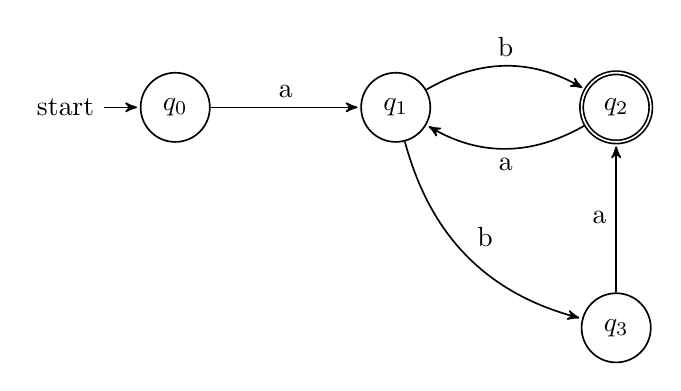
\begin{tikzpicture}[->,>=stealth',shorten >=1pt,auto,node distance=2.8cm,
                    semithick]
  % \tikzstyle{every state}=[fill=red,draw=none,text=white]

  \node[initial,state] (A)                    {$q_0$};
  \node[state]         (B) [right of=A] {$q_1$};
  \node[state,accepting]         (C) [right of=B] {$q_2$};
  \node[state]         (D) [below of=C] {$q_3$};

  \path (A) edge                      node {a} (B)
            (B) edge [bend left]     node {b} (C)
                edge [bend right]   node {b} (D)
        (C) edge [bend left]        node {a} (B)
        (D) edge                        node {a} (C);
\end{tikzpicture}
\end{document}
